\documentclass[12pt]{article}
\usepackage[utf8]{inputenc}

\usepackage{lmodern}

\usepackage{enumitem}
\usepackage[margin=2cm]{geometry}

\usepackage{amsmath, amsfonts, amssymb}
\usepackage{graphicx}
%\usepackage{subfigure}
\usepackage{tikz}
\usepackage{pgfplots}
\usepackage{multicol}

\usepackage{comment}
\usepackage{url}
\usepackage{calc}
\usepackage{subcaption}
\usepackage[indent=0pt]{parskip}
\usepackage{animate}

\usepackage{array}
\usepackage{blkarray,booktabs, bigstrut}
\usepackage{bigints}

\pgfplotsset{compat=1.16}

% MATH commands
\newcommand{\ga}{\left\langle}
\newcommand{\da}{\right\rangle}
\newcommand{\oa}{\left\lbrace}
\newcommand{\fa}{\right\rbrace}
\newcommand{\oc}{\left[}
\newcommand{\fc}{\right]}
\newcommand{\op}{\left(}
\newcommand{\fp}{\right)}

\newcommand{\bi}{\mathbf{i}}
\newcommand{\bj}{\mathbf{j}}
\newcommand{\bk}{\mathbf{k}}
\newcommand{\bF}{\mathbf{F}}

\newcommand{\mR}{\mathbb{R}}

\newcommand{\ra}{\rightarrow}
\newcommand{\Ra}{\Rightarrow}

\newcommand{\sech}{\mathrm{sech}\,}
\newcommand{\csch}{\mathrm{csch}\,}
\newcommand{\curl}{\mathrm{curl}\,}
\newcommand{\dive}{\mathrm{div}\,}

\newcommand{\ve}{\varepsilon}
\newcommand{\spc}{\vspace*{0.5cm}}

\DeclareMathOperator{\Ran}{Ran}
\DeclareMathOperator{\Dom}{Dom}

\newcommand{\exo}[1]{\noindent\textcolor{red}{\fbox{\textbf{Problem {#1}}}\hrulefill}\\}
\newcommand{\qu}[4]{\noindent\textcolor{#4}{\fbox{\textbf{Section {#1} | Problem {#2}}} \hrulefill{{\fbox{\textbf{{#3} Points}}}}\\}}

\newcommand{\semester}{Spring 2023}

\newcommand{\CVup}{%

\begin{tikzpicture}
\draw[black, <->, >=latex] (-0.33, 0.5) .. controls (-0.125, 0) and (0.125, 0) .. (0.33, 0.5);
\end{tikzpicture}}

\newcommand{\CVupInc}{%
\begin{tikzpicture}
\draw[black, ->, >=latex] (0,0) .. controls (0.2, 0) and (0.4, 0.2) .. (0.5, 0.5);
\end{tikzpicture}}

\newcommand{\CVupDec}{%
\begin{tikzpicture}[rotate=270]
\draw[black, ->, >=latex] (0,0) .. controls (0.2, 0) and (0.4, 0.2) .. (0.5, 0.5);
\end{tikzpicture}}

\newcommand{\CVdown}{%
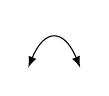
\begin{tikzpicture}
\draw[black, <->, >=latex] (-0.33, -0.5) .. controls (-0.125, 0) and (0.125, 0) .. (0.33, -0.5);
\end{tikzpicture}}

\newcommand{\CVdownInc}{%
\begin{tikzpicture}
\draw[black, ->, >=latex] (-0.5, -0.5) .. controls (-0.5, -0.3) and (-0.5, -0.1) .. (0,0);
\end{tikzpicture}}

\newcommand{\CVdownDec}{%
\begin{tikzpicture}[rotate=-90]
\draw[black, ->, >=latex] (-0.5, -0.5) .. controls (-0.5, -0.3) and (-0.5, -0.1) .. (0,0);
\end{tikzpicture}}

\begin{document}
	\noindent \hrulefill \\
	MATH-241 \hfill Pierre-Olivier Paris{\'e}\\
	Solutions Section 4-1 \hfill \semester \\\vspace*{-1cm}
	
	\noindent\hrulefill
	
	\spc

	\exo{4}
	\begin{enumerate}
	\item[a)] We have $n = 4$ and so $\Delta x = (\pi/2 - 0)/4 = \pi/8$. The sample points are
		\begin{align*}
		x_1 = \pi/8 , \, x_2 = \pi/4 , \, x_3 = 3\pi/8 , \, x_4 = \pi/2 .
		\end{align*}
	So, we obtain
		\begin{align*}
		A &\approx \sin (\pi/8) \Delta x + \sin (\pi/4) \Delta x + \sin (3\pi/8) \Delta x + \sin (\pi/2 ) \Delta x \\
		& = (\pi/8) (\sin (\pi/8) + \sin (\pi/4) + \sin (3\pi/8) + \sin (\pi/2) ) \\
		& \approx 1.18346 .
		\end{align*}
	Here is the graph of the function and the approximate squares. We see that we overestimated the area under the curve.
		\begin{figure}[ht]
		\centering
		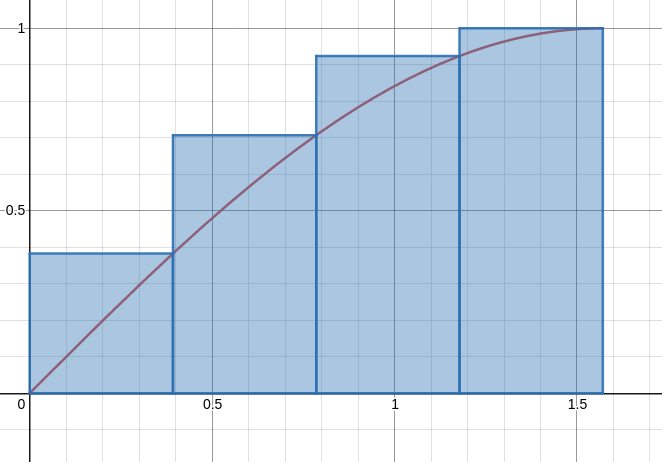
\includegraphics[scale=0.3]{RiemannSums.png}
		\end{figure}
	
	\item[b)] We have $n = 4$ and so $\Delta x = (\pi/2 - 0)/4 = \pi/8$. The sample points are
		\begin{align*}
		x_1 = 0, \, x_2 = \pi/8 , \, x_3 = \pi/4 , \, x_4 = 3\pi/8 .
		\end{align*}
	We then obtain
		\begin{align*}
		A &\approx \sin (0) \Delta x + \sin (\pi/8 ) \Delta x + \sin (\pi/4 ) \Delta x + \sin (3\pi/8 ) \Delta x \\
		&= (\pi/8 ) (\sin (0) + \sin (\pi/8 ) + \sin (\pi/4 ) + \sin (3\pi/8 ) )  \approx 0.790766 .
		\end{align*}
	Here is the graph of the function and the approximate squares. 	We see that we overestimated the area under the curve.
		\begin{figure}[ht]
		\centering
		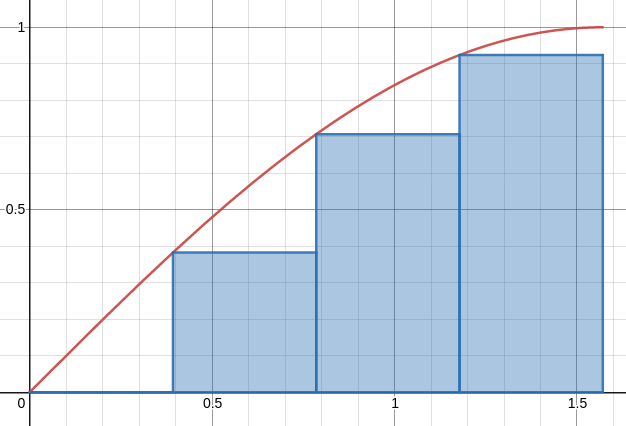
\includegraphics[scale=0.3]{Number4_41.png}
		\end{figure}

	\end{enumerate}
	
	\spc
	
	\exo{14 (except c))}
	\begin{enumerate}
	\item[a)] We have $t_1 = 0$, $t_2 = 10$, $t_3 = 20$, $t_4 = 30$, $t_5 = 40$, and $t_6 = 50$ as our sample points and $\Delta x = 10$. So, the distance is estimated by
		\begin{align*}
		10(182.9) + 10(168.0) + 10(106.6) + 10(99.8)+10(124.5)+10(176.1) \approx 8579.0 \text{ miles.}
		\end{align*}
	\item[b)] We have this time $t_1 = 10$, $t_2 = 20$, $t_3 = 30$, $t_4 = 40$, $t_5 = 50$, and $t_6 = 60$ as our sample points and $\Delta x = 10$. So, the distance is estimated by
		\begin{align*}
		10(168.0) + 10(106.6) + 10(99.8) + 10(124.5) + 10(176.1) + 10(175.6) \approx 8506.0 \text{ miles.}
		\end{align*}
	\end{enumerate}
	
\end{document}